\section*{\color{SectionBlue}{Analysis}} \label{sec:sections}
\addcontentsline{toc}{section}{Analysis}
\subsection*{\color{SubSectionBlue}{Hyperparameters}}
\addcontentsline{toc}{subsection}{Hyperparameters} \\

Throughout this research, there were two major changes that distinguished Quantum Save when compared to existing algorithms. The first is the utilization of quantum computing, or the IBM Q32 quantum simulator. To evaluate the effectiveness of quantum computing in optimizing the Knapsack problem, or more accurately the cybersecurity defense problem, the evolution of Quantum Save was compared to that of Kucharski and Nowotniak \cite{nowotniak_higher-order_2014}. 
Kucharski and Nowotniak \cite{nowotniak_higher-order_2014} used a classical implementation of the quantum-inspired genetic algorithm to find a solution to the knapsack problem.In order to establish the significance of Quantum Save in the context of the Knapsack problem, the baseline optimization that was obtained, without any probability amplitude manipulation, was compared to the highest value obtained by Nowotniak and Kucharski \cite{nowotniak_higher-order_2014}, \$5709.

\vspace{1mm}

In order to compare the results of Quantum Save when compared to previous research, a 1-sample t-test with a significance level of 0.05 was run on the baseline probability manipulation (Table 1) and the results of the test were used to determine whether Quantum Save on the IBM Q32 simulator was significantly better when compared to Kucharski and Nowotniak \cite{nowotniak_higher-order_2014}. Since both of the p-values (one-tailed and two-tailed) obtained from the 1-sample t-test, \textit{0.003} and \textit{0.005} respectively, were less than the established significance level of 0.05, the null hypothesis could be confidently rejected. If the null hypothesis was true, as the proposed algorithm didn’t perform any better than that of previous research, there would only be a 0.274 or 0.548 percent chance of obtaining a profit value this high or higher based upon random sampling variability alone. Therefore, there is enough statistical evidence to suggest that Quantum Save on the IBM Q32 computer performed significantly better than that of previous research. In the end, Quantum Save, on the IBM quantum simulators, likely performed better due to the simulation of more qubits and the existence of four quantum chromosomes in the population as opposed to three. These factors allowed for more genetic variability and increased the chance of finding the non-obvious solutions to the knapsack problem. Different routes were taken and ultimately, a higher optimization of the knapsack function was achieved. 

\vspace{1mm}

However, Quantum Save was improved by tuning hyper parameter values including the value of µ which described the amount of probability amplitude manipulation and the generation for which to implement the disaster algorithm. First, when regarding the manipulation of probability amplitudes, an analysis of variance test, or an ANOVA test, was run to determine whether the change in probability amplitudes did in fact achieve a statistically significant change in the optimization of the knapsack problem. The significance level of the ANOVA test was 0.10 and that represented the alpha power of this statistical test. When implementing the probability amplitude manipulation, the goal was to simply increase the optimization of the knapsack problem. So, the alpha power of the test did not need to be extremely high so a value of 0.1 was chosen. Since the p-value of \textit{.052} is less than the significance level of 0.1, the null hypothesis could be confidently rejected. If the null hypothesis was true, as the proposed algorithm with manipulation of amplitudes did not perform any better than the algorithm without the manipulation of amplitudes, there would only be a 5.27\% chance of obtaining a profit value this high or higher based upon random sampling variability alone. Therefore, there is enough statistical evidence, within the power of this ANOVA test, to suggest that the manipulation of probability amplitudes increased the optimization of the knapsack problem. Since the ANOVA test does not provide the greatest value for µ, that had to be calculated manually. When looking at the data table, it could be observed that a µ value of 0.9 or a 90\% manipulation of amplitudes resulted in the highest optimization of the knapsack problem. In order to confirm the values obtained from the ANOVA test, the maximum profit over the probability amplitudes were observed. 

\vspace{1mm}

The second tuned hyper parameter was the generation on which to implement the disaster algorithm. To determine whether the disaster algorithm achieved a statistically significant change in the optimization of the Knapsack problem, another analysis of variance test, or an ANOVA test, was run. Again, like with the manipulation of probability amplitudes, the the significance level of the ANOVA test was 0.10 and that represented the alpha power of this statistical test. With a p-value of \textit{0.848}, it appears that the disaster algorithm does not significantly increase the optimization of the Knapsack problem. However, in Table 1, a disaster step of 6 does increase the optimization of the knapsack problem by around 3.22\%. Although this is not statistically significant, there is some improvement. The disaster algorithm will help only when Quantum Save reaches a local maxima, which might not occur in every  trial. So, with any improvement, the disaster algorithm is considered successful. Also, when looking at Table 1, the standard error with the disaster algorithm is much lower when compared to the baseline. This suggests that the disaster algorithm is preventing Quantum Save from getting caught on the lower local maxima. Now, the probability of finding that non-obvious solution increases drastically. 

\subsection*{\color{SubSectionBlue}{Accuracy of Quantum Save}}
\addcontentsline{toc}{subsection}{Accuracy of Quantum Save} \\

The second uniqueness of Quantum Save when compared to previous research, such as the linear optimization model \cite{rakes_it_2012} is the implementation of the QGA algorithm in cybersecurity budget allocation. However, when analyzing the effectiveness of Quantum Save in the realm of cybersecurity budget allocation, there are two distinct features that need to be considered: the accuracy and the run time. With the accuracy, the budget allocation techniques of Quantum Save can be compared with the techniques from linear optimization models \cite{rakes_it_2012}. The techniques will be quantified by analyzing the amount of money that a small-medium target will lose when implementing the countermeasures suggesting by each respective algorithm. The better algorithm will be the one that results in lower monetary loss in the case of an attack by foreign or domestic adversaries. From a simple eye-test on the data presented in Table 2, it appeared that my algorithm performed better when compared to previous research \cite{rakes_it_2012} at every budget range. However, the extent of that improvement varied significantly (Table 3).

\begin{singlespace}
\vspace*{0.6cm}
\begin{table}[H]
    \centering
    \caption{Percent Improvement by Quantum Save}
    \label{parametri}
    \resizebox{0.27\textwidth}{!}{%
    \begin{tabular}{@{}1l@{}}
    \toprule
    Budget & \% Improvement \\ \midrule
    80k & 17.48 \\
    108k & 0.24 \\
    132k & 6.53 \\
    148k & 0.05 \\
    158k & 9.19 \\
    178k & 4.42 \\
    \bottomrule
    \end{tabular}}
\end{table}
\end{singlespace}
\addcontentsline{toc}{subsubsection}{Table 3: Percent Improvement by Quantum Save} \\

When looking at Table 3, it was determined that Quantum Save performed better when compared to the generalized linear optimization model. But, the extent of that improvement varied from 0.05\% to 17.48\%. Since the discrepancy in the percent improvement is so high, another statistical method had to be taken to ensure that the improvement was not caused by random variability. The distribution of Quantum Save's outputs at each budget range was analyzed using a box plot (Figure 10).

\begin{figure}[ht]%
\centering
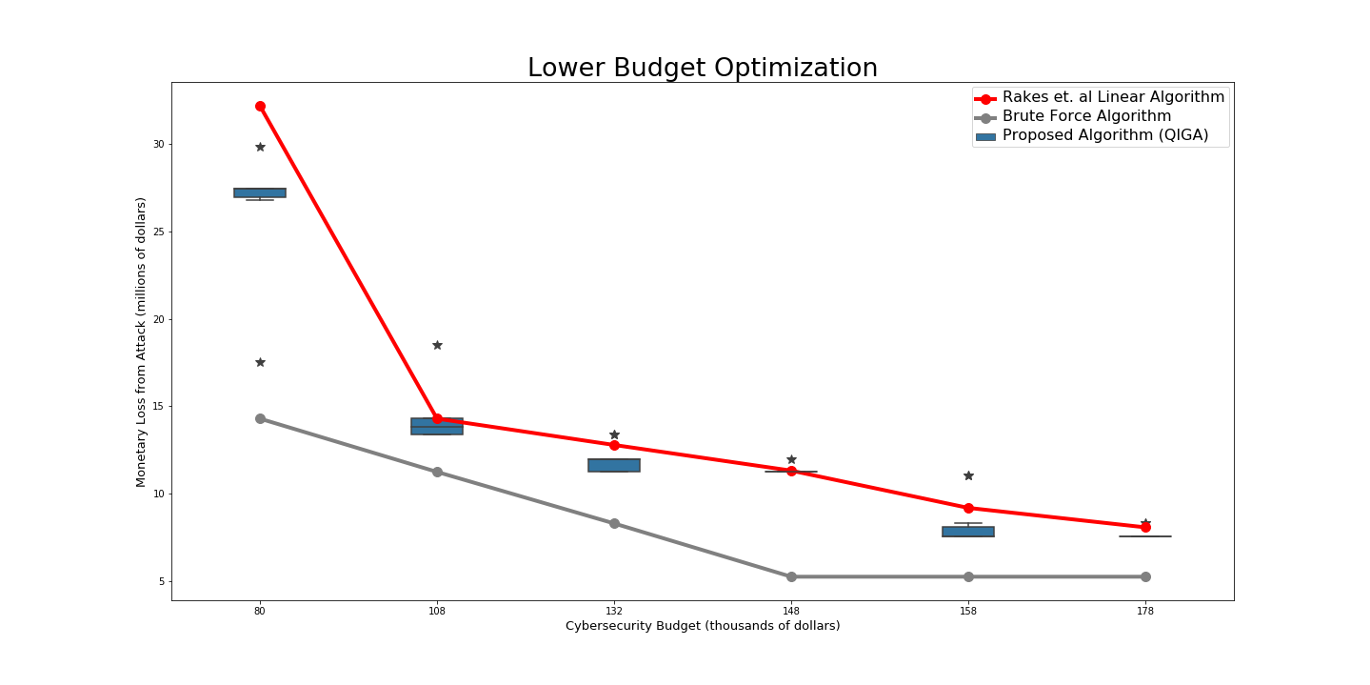
\includegraphics[width=11cm,height=5.6cm]{Images/boxplot.png}
\caption{Distribution of Quantum Save's Results by Budget}%
\end{figure}
\addcontentsline{toc}{subsubsection}{Figure 10: Distribution of Quantum Save's Results by Budget} 

When analyzing the box plot, data points that were outside of a standard 95\% confidence interval, or a 1.57 IQR range were labeled as outliers (as can be seen by the stars on the box plot). So, based upon the distribution of outputs shown in the box plot, barring outliers, it appears as if Quantum Save's results for the expected-case number of attacks per year were either less than or equal to the linear optimization mode. \cite{rakes_it_2012}. Although in some budgets Quantum Save allocated budgets as effectively as the linear model, that still serves to emphasize the significance of Quantum Save in the realm of allocating cybersecurity budgets. 

\subsection*{\color{SubSectionBlue}{Time Complexity of Quantum Save}}
\addcontentsline{toc}{subsection}{Time Complexity of Quantum Save} \\

The second technique for analyzing the uniqueness in Quantum Save when compared to previous research, such as the linear optimization model proposed by Rakes et al. \cite{rakes_it_2012}. In typical countermeasure recommendation lists, there are approximately 50 to a 100 countermeasures meaning any algorithm that attempts to allocate cybersecurity budgets needs to scale well. Using an algorithm which scales exponentially would be extremely time consuming, which is a luxury that most smaller-medium targets can not afford. Instead, a cybersecurity budget allocation algorithm needs to be able to produce high number countermeasure recommendation lists in a reasonable amount of time. To ensure that Quantum Save could meet that criteria, the run time of the algorithm was measured. The data was then analyzed by finding both an experimental and theoretical relationship between the number of countermeasures in the recommendation list and the run time of the algorithm. When considering experimental data, the run time of both a traditional brute force algorithm and Quantum Save was charted. Brute force was chosen as a comparison algorithm because it has the best accuracy of any potential cybersecurity budget allocation problem. 

\begin{figure}[ht]%
    \centering
    \subfloat[Quantum Save Time Complexity]{{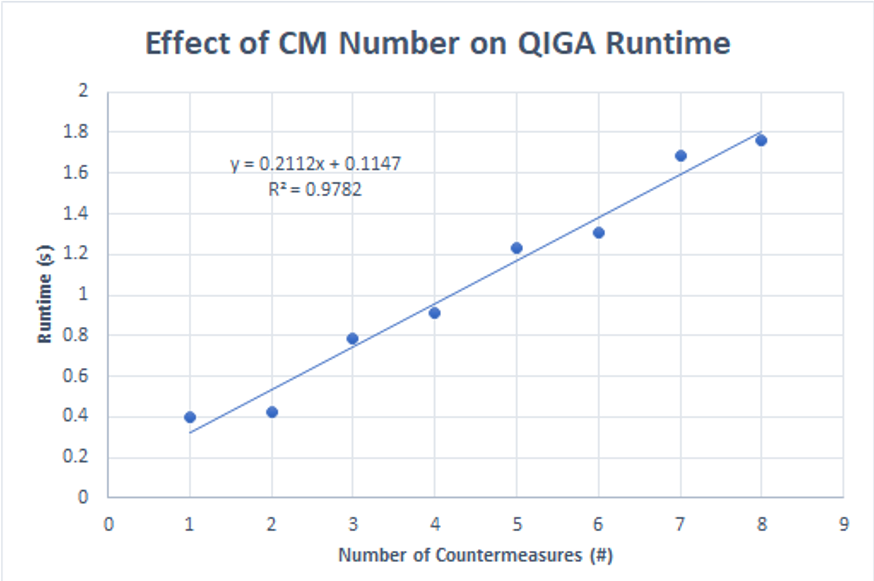
\includegraphics[width=7.65cm]{Images/q-save-runtime.png} }}%
    \qquad
    \subfloat[Brute Force Time Complexity]{{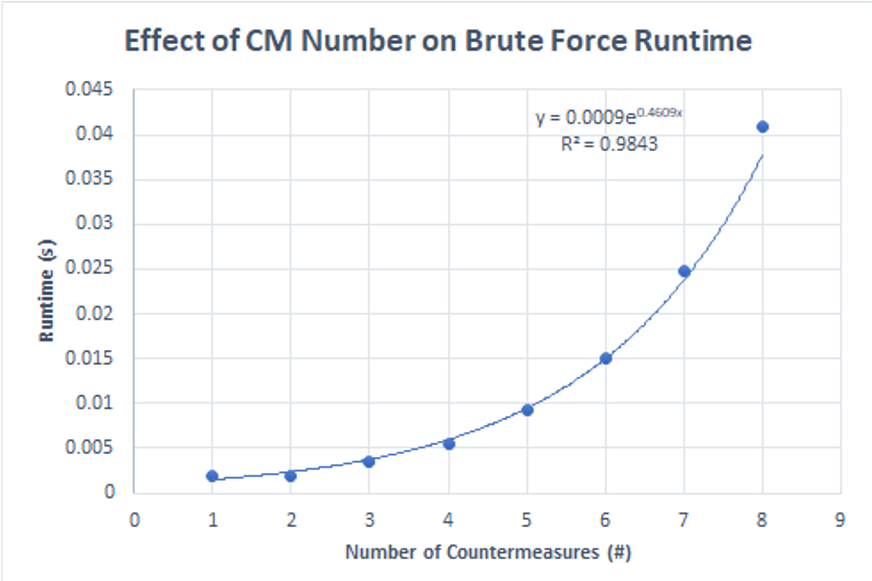
\includegraphics[width=7.65cm]{Images/brute-force-runtime.png} }}%
    \caption{Time Complexity of Quantum Save vs. Brute Force}%
    \label{fig:example}%
\end{figure}
\addcontentsline{toc}{subsubsection}{Figure 11: Time Complexity of Quantum Save vs. Brute Force} \\

The run time results, which showed the relationship between the run time of a Brute Force algorithm and the size of the input, was fitted with an exponential trend line and an r-squared value of 0.9843 was obtained. This high r-squared value suggests that 98.43\% of the variation in the run time of the algorithm was explained by the difference in input size, or the difference in the size of the countermeasure recommendation lists. The experimental results makes sense since Brute Force algorithms generally scale exponentially. This replication of Brute Force scalability provides justification for using this experimental method of determining run time. The other pair of results results, which showed the relationship between Quantum Save's run time and the size of the input, was fitted with a linear trend line and an r-squared value of 0.9782 was obtained. Again, this high r-squared value suggests that 97.82\% of the variation in the run time of the algorithm was explained by the difference in input size, or the difference in the size of the countermeasure recommendation lists. This experimental data provides an initial suggestion that the algorithm scales linearly, but a theoretical justification is needed to supplement the idea. 

\begin{lemma}
Quantum Save can allocate budget, $b$, when choosing from countermeasures with input-size, $n$, in $\mathcal{O}(n)$ time complexity with oracles for quantum measurement of a single register.
\end{lemma}

\begin{proof}
In the first line of Algorithm 2, the first phase of Quantum Save, the number of countermeasures is defined. This definition directly depends upon the input-size of the recommendation list, resulting in a complexity of $\mathcal{O}(n)$. From lines 2 - 4, basic variables for Quantum Save are defined. Since these variables are not correlated to the input-size, the resulting complexity is $\mathcal{O}(1)$. In line 5 - 6, the first loop begins which loops through the number of generations and the quantum register variable gets initialized. Again, since the number of generations is not correlated to the input-size, the resulting complexity of these lines is $\mathcal{O}(1)$. In line 7, a second loop begins which loops through every quantum register in the population. Since the quantum registers depend on the input size, these lines have a complexity of $\mathcal{O}(n)$. In lines 8 - 11, the quantum circuit is created and measured. Since the measurement of a single register does not depend on the size of the input, these lines have a complexity of $\mathcal{O}(1)$. Because the highest complexity is $\mathcal{O}(n)$ and there are no nested loops of higher complexity, the complexity of the first phase is $\mathcal{O}(n)$.

\vspace{1mm}

In the first two lines of Algorithm 3, the second phase of Quantum Save, the CISO variable is initialized and all of the CISO's are looped through. Since the number of CISO's does not vary based upon input size, the complexity of these lines is $\mathcal{O}(1)$. After a couple of definitions, which are $\mathcal{O}(1)$, the results of the quantum measurement are looped through in line 5. Since the job string would be longer if there are more countermeasures in the input, the complexity of this lines is $\mathcal{O}(n)$. Next, after a couple more definitions, which again are $\mathcal{O}(1)$, each countermeasure in the input array is looped through in line 9. Since the input array directly correlates with input-size, the complexity of this lines is $\mathcal{O}(n)$. Finally, in line 14, the maximum profit value produced is determined. Since the number of CISO remains constant, the complexity of this line is $\mathcal{O}(1)$. Because the highest complexity is $\mathcal{O}(n)$ and there are no nested loops of higher complexity, the complexity of the second phase is $\mathcal{O}(n)$.

\vspace{1mm}

After the definitions in the first two lines of Algorithm 4, which are $\mathcal{O}(1)$, the CISO's in the populationa re looped through. Since the number of CISO's does not vary based upon input size, the complexity of line 3 is $\mathcal{O}(1)$. Next, after a definition in line 4, line 5 of Quantum Save loops through every countermeasure in the binary array. Since the binary array increases with direct proportionality to the size of the inputs, the complexity of this line is $\mathcal{O}(n)$. Finally, the manipulation of the probability amplitudes, in lines 6 - 8, have a complexity class of $\mathcal{O}(1)$. Because the highest complexity is $\mathcal{O}(n)$ and there are no nested loops of higher complexity, the complexity of the third phase is $\mathcal{O}(n)$.

\vspace{1mm}

Since the complexity of all three phases are $\mathcal{O}(n)$, the final time complexity for Quantum Save is $\mathcal{O}(n)$. So, Quantum Save can allocate budget, $b$, when choosing from countermeasures with input-size, $n$, in $\mathcal{O}(n)$ time complexity with oracles for quantum measurement of a single register.
\end{proof}

From both the theoretical and the experimental justifications, it can be determined that Quantum Save is an algorithm that scales linearly and this quality would be extremely helpful in developing large countermeasure recommendation lists that is typical in the industry.

